\documentclass{beamer}

% \usetheme{Pittsburgh}
 \setbeamertemplate{enumerate items}[circle]
%  \usetheme{Boadilla}
\usepackage[ngerman,english]{babel}			
\usepackage[utf8]{inputenc}				

\usepackage{color}
% \usepackage[table,x11names]{xcolor}
\usepackage{booktabs}
\usepackage{animate}
\usepackage{hyperref}
\usepackage{dirtytalk} % quotes
\usepackage{amsmath}
\usepackage{bm}

% \usepackage{natbib}
% \usepackage{apalike}
% \bibliography{refs}

\usepackage[style=apa]{biblatex}
\addbibresource{refs.bib}

% Define command to print full bibliography in footnote
\newcommand{\fcite}[1]{\footnote{\fullcite{#1}}}

\hypersetup{colorlinks,urlcolor=blue, linkcolor=blue}

\setbeamertemplate{footline}[frame number]
\setbeamertemplate{section in toc}[sections numbered]
\setcounter{tocdepth}{2}
% \setbeamertemplate{subsection in toc}[subsections numbered]

% LOGO TOP RIGHT
% \usepackage{tikz}
% \titlegraphic { 
% \begin{tikzpicture}[overlay,remember picture]
% \node[left=0.2cm] at (current page.30){
%     
\includegraphics[width=3cm]{figures/mpidr_logo_colour_de_1.png}
% };
% \end{tikzpicture}
% }

% LOGO BOTTOM RIGHT
\titlegraphic{

\includegraphics[width=5cm]{figures/mpidr_logo_colour_de_1.png}
\hfill

\includegraphics[width=3cm]{figures/edsd-logo.png}
}

% \makeatletter
% \setbeamertemplate{navigation symbols}{}

% make blocks no transparent
\setbeamercolor{block body alerted}{bg=alerted text.fg!10}
\setbeamercolor{block title alerted}{bg=alerted text.fg!20}
\setbeamercolor{block body}{bg=structure!10}
\setbeamercolor{block title}{bg=structure!20}
\setbeamercolor{block body example}{bg=green!10}
\setbeamercolor{block title example}{bg=green!20}



%%	title page information

\title[Kinship]{Kinship Structures (2)}
\subtitle{The formal demography of kinship}

\author{Diego Alburez Guti\'errez$^{\dagger}$}

\institute{$^{\dagger}$Kinship Inequalities Research Group, \\ Max Planck Institute for Demographic Research }

\date{European Doctoral School of Demography 2025-26 \\ 3 Mar 2026}

%%	Begin of the document:
%%	======================

\begin{document}

 \begin{frame}[t,plain]
 \titlepage
 \end{frame}

 
\begin{frame}{Agenda}
\tableofcontents
\end{frame}

\begin{frame}{What are kinship models?}
    \begin{enumerate}
        \item Kinship is an \textit{emergent property} of demographic systems
        \item Simplified representation of interaction between reproduction and death 
        \item Not restricted to humans\fcite{coste_kinship_2021}
    \end{enumerate}
    
    \vspace{.7cm}
    
    $\rightarrow{}$ What are emergent properties?\\
    $\rightarrow{}$ Can you think of other emergent properties in nature, society, or demography?
\end{frame}

\begin{frame}{Formal models of kinship}

Given a set of:
\vspace{0.2cm}
    \begin{itemize}
        \item age-specific fertility rates 
        \item survival probabilities
        \item simplifying assumptions
    \end{itemize}
\vspace{0.5cm}

The models produce:
\vspace{0.2cm}
\begin{enumerate}
    \item Number of (living/dead) kin
    \item Age distribution of relatives
    \item From the point of view of an average member of the population (`Focal')
\end{enumerate}
\end{frame}

\begin{frame}{Focal: an average member of the population}
      \begin{figure}[!h]
      \centering
      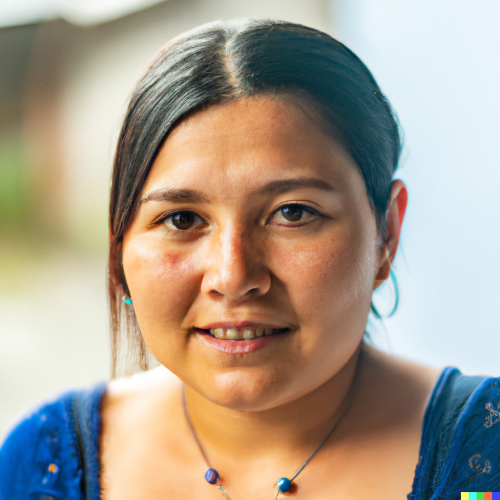
\includegraphics[width =.7\textwidth]{figures/focal.png}
     \end{figure}    
\end{frame}

\begin{frame}{Typology of kinship models}

\begin{table}[]
\begin{tabular}{@{}lllll@{}}
\toprule
No & time      & sex    & state    & reference \\ \midrule
\textbf{1} & \textbf{invariant} & \textbf{female} & \textbf{age} & \fcite{caswell_formal_2019}          \\ 
2 & variant   & female & age & \fcite{caswell_formal_2021}           \\
3 & invariant & two   & age & \fcite{caswell_formal_2022}          \\
4 & invariant   & female   &  multiple & \fcite{caswell_formal_2020}  \\ 
5 & variant   & two   &  multiple & \fcite{williams_demokin_2023}  \\ \bottomrule
\end{tabular}
\end{table}

\end{frame}

\begin{frame}{Model characteristics}
    
    Define the following model characteristics:
    \vspace{0.3cm}
    
    \begin{enumerate}
        \item Time-(in)variance
        \item One/two-sex models
        \item (Multi)state models
    \end{enumerate}
    
\end{frame}

\section{The Goodman-Keyfitz-Pullum kinship equations}
\begin{frame}
    \begin{centering}
    \begin{beamercolorbox}[sep=12pt,center]{part title}
    \usebeamerfont{section title}\insertsection\par
    \end{beamercolorbox}
    \end{centering}
\end{frame}


\begin{frame}{The tree of life}
       \begin{figure}[!h]
       \centering
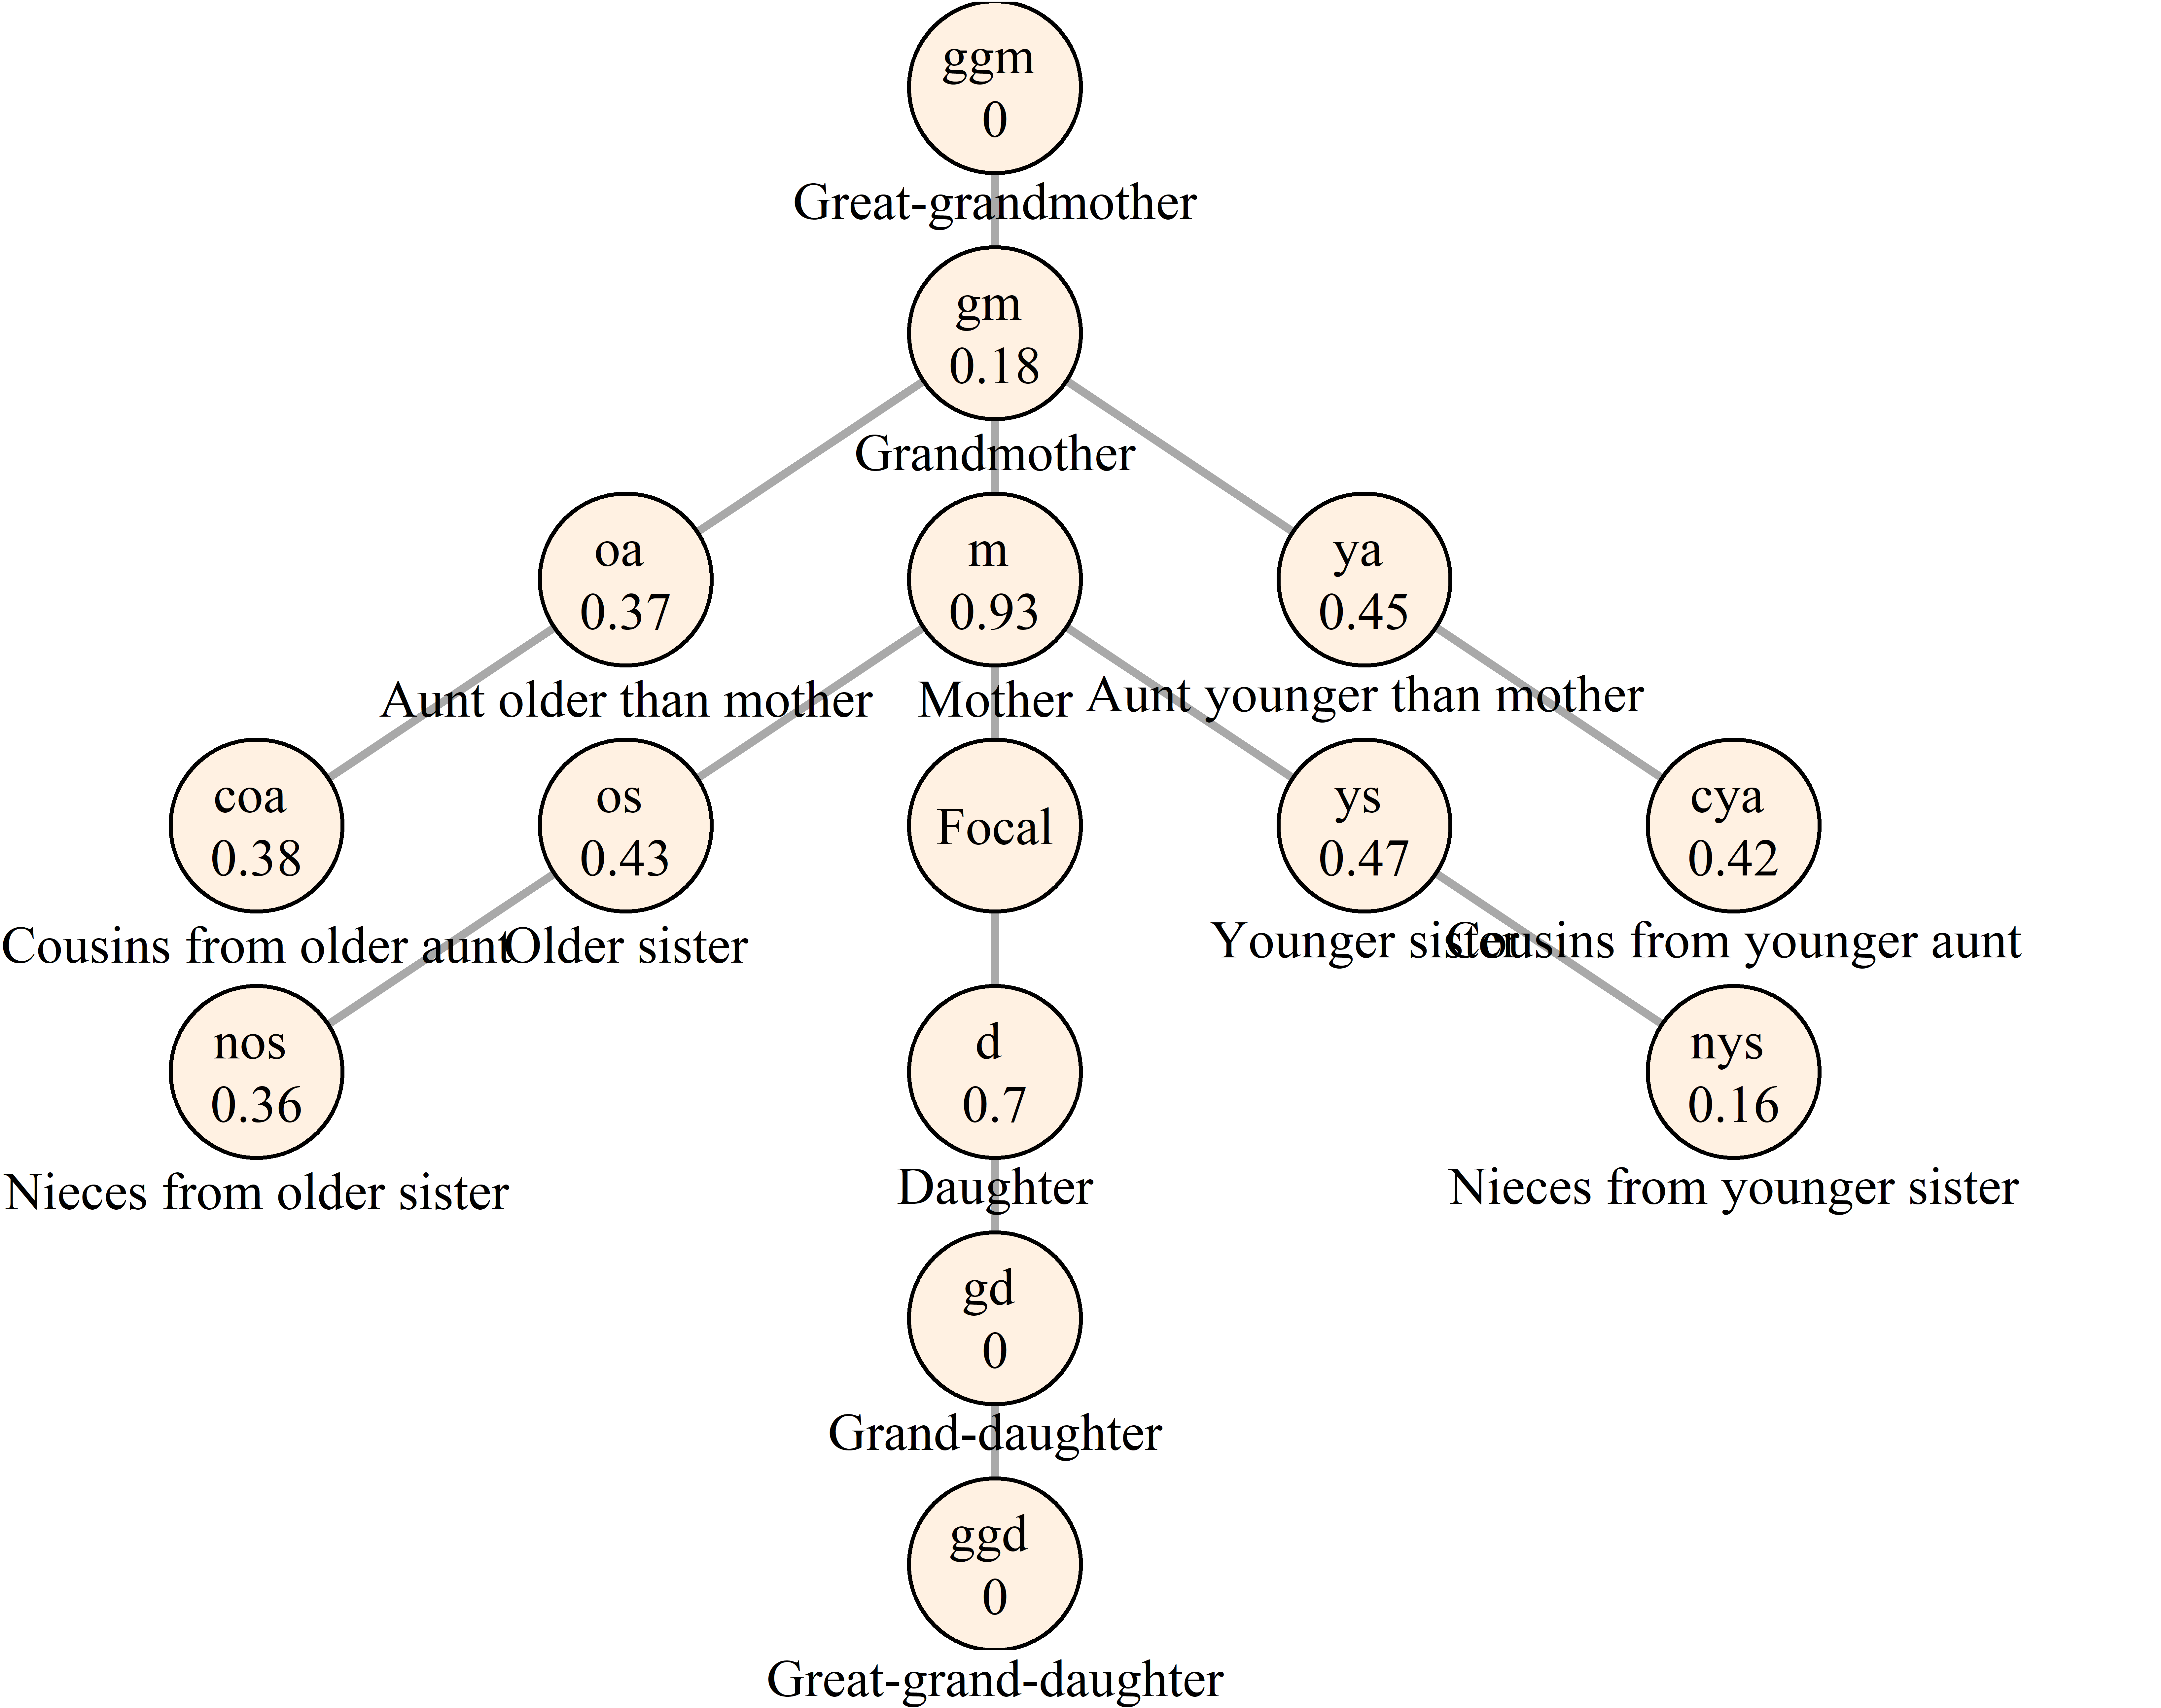
\includegraphics[width =1\textwidth]{figures/tree.png}
     \end{figure}
\end{frame}

\begin{frame}{Expected number of kin}
    \begin{figure}[!h]
       \centering
        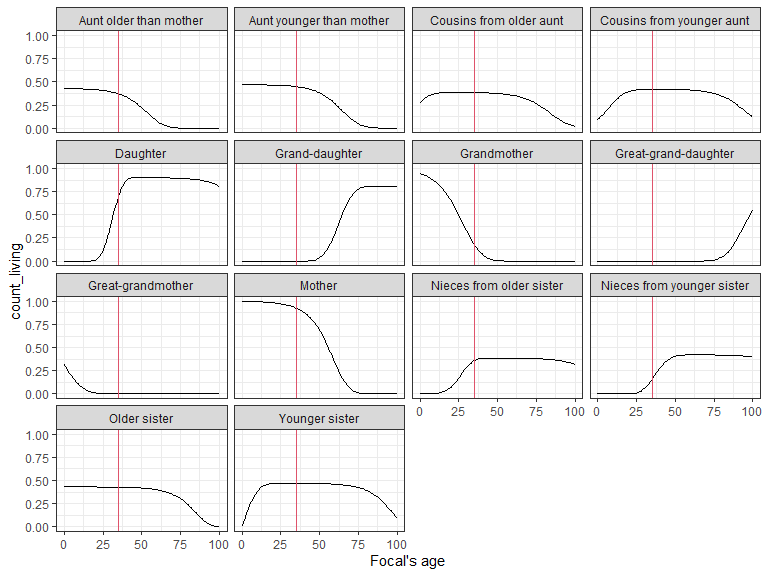
\includegraphics[width =1\textwidth]{figures/kin1.png}
     \end{figure}
\end{frame}

\begin{frame}{Daughters}
    
    $B_1(a)$ is the expected number of living daughters in a time-invariant female-only population\fcite{goodman_family_1974}:
    
\begin{equation}
B_1(a) = \int_{\alpha}^{a}{m(x) l(a-x) \: dx}
\label{eq:b1}
\end{equation}

where:

\begin{itemize}
    \item $m(x)$ are fertility rates of mothers
    \item $l(a-x)$ are survival probabilities of daughters
\end{itemize}
    
\end{frame}

\begin{frame}{Daughters}
    
If $a = 20$ and $\alpha = 15$; then:

\begin{equation*}
B_1(20) \approx \sum_{15}^{20}{m(x) l(20-x)}
\end{equation*}

So...

\begin{equation*}
B_1(20) \approx m(15)l(5) + m(16)l(4) + m(17)l(3) \ldots
\label{eq:b1}
\end{equation*}
    
\end{frame}

\begin{frame}{Granddaughters}
    
$B_1(a)$ is the expected number of living granddaughters in a time-invariant female-only population\fcite{goodman_family_1974}:
    
\begin{equation}
B_2(a) = \int_{\alpha}^{a}{m(x)\int_{\alpha}^{a-x}{l(y) m(y) l(a-x-y) \: dy }\:dx} 
\label{eq:b2}
\end{equation}
    
\end{frame}

\begin{frame}{}
       \begin{figure}[!h]
       \centering
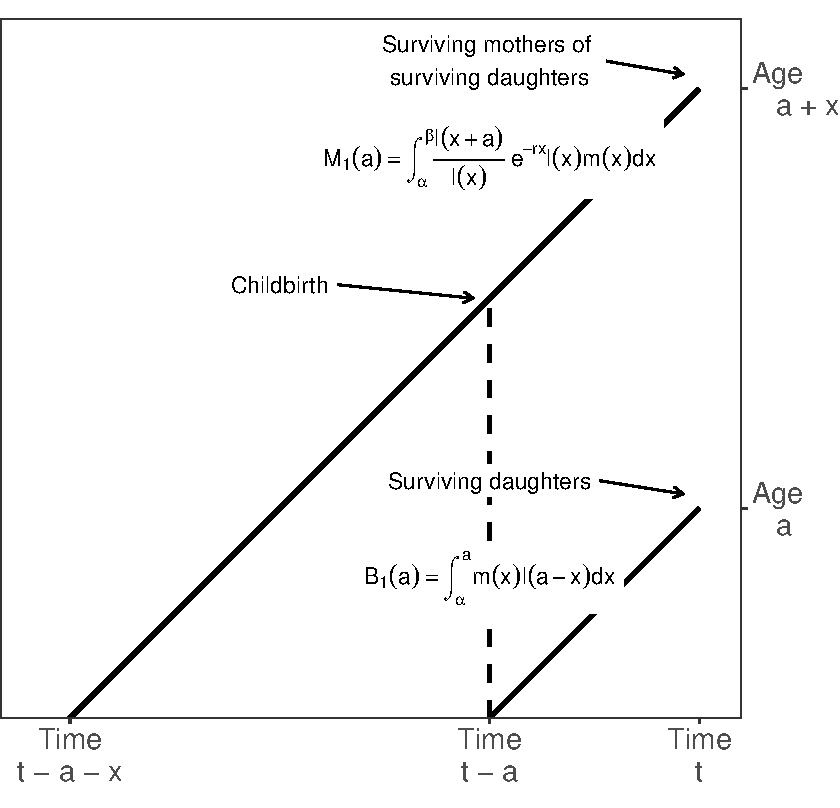
\includegraphics[width =.8\textwidth]{figures/lexis.pdf}
     \end{figure}
\end{frame}

\begin{frame}{Mothers}
    
$M_1(a)$ is the probability of having a living mother in a time-invariant female-only population\fcite{goodman_family_1974}:

\begin{equation}
% M_1(a) = \int_{\alpha}^{\beta}{ \underbrace{\frac{l(x+a)}{l(x)}}_{\substack{\text{prob of surviving}\\ \text{from $x$ to $a+x$}}} \times \underbrace{e^{-rx}l(x)m(x)}_{\substack{\text{age distribution of}\\ \text{mothers}}}  dx}.
M_1(a) = \int_{\alpha}^{\beta}{ \underbrace{\frac{l(x+a)}{l(x)}}_{\substack{\text{prob of surviving}\\ \text{from $x$ to $a+x$}}} \times \underbrace{W(x)}_{\substack{\text{age distribution of}\\ \text{mothers}}}  dx}.
\label{eq:m1a}
\end{equation}

where:

\begin{itemize}
    \item $W(x) = e^{-rx}l(x)m(x)$ is the age distribution of mothers
    \item $l(x)$ are survival probabilities
    \item $m(x)$ are fertility rates
    \item $r$ is the population growth rate
    \item $\alpha$-$\beta$ is the reproductive period
\end{itemize}

\end{frame}

\begin{frame}{}
       \begin{figure}[!h]
       \centering
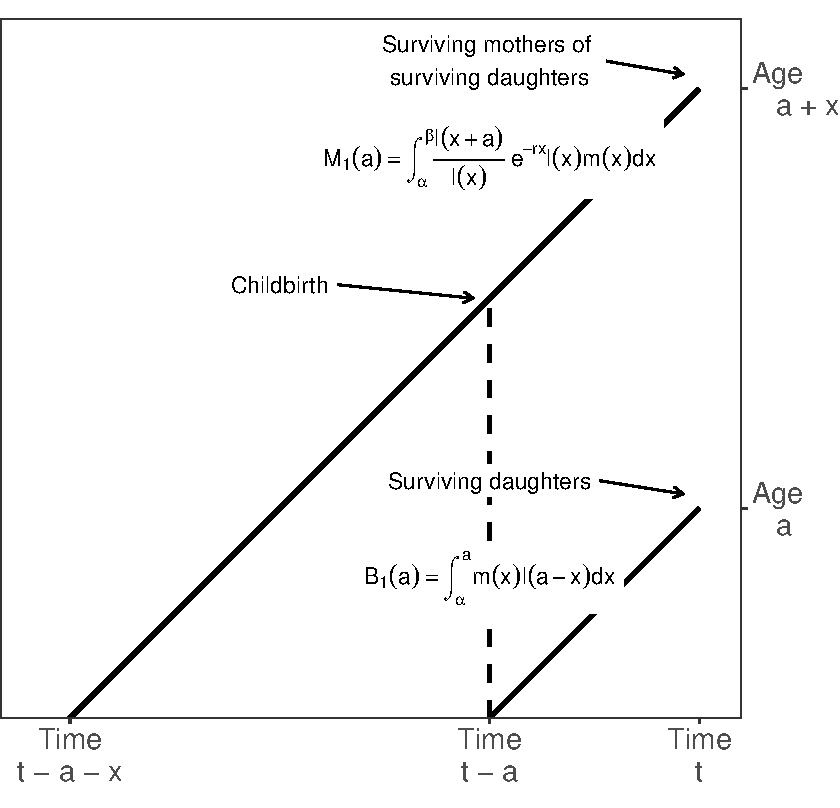
\includegraphics[width =.8\textwidth]{figures/lexis.pdf}
     \end{figure}
\end{frame}

\begin{frame}{Grandmothers}
    
$M_2(a)$ is the expected number of living grandmothers in a time-invariant female-only population\fcite{goodman_family_1974}:

\begin{equation}
% M_2(a) = \int_{\alpha}^{\beta}{ \underbrace{ \textcolor{red}{M_1(a)} }_{\substack{\text{prob of having}\\ \text{living mother}}} \times \underbrace{e^{-rx}l(x)m(x)}_{\substack{\text{age distribution of}\\ \text{mothers}}}  dx}.
M_2(a) = \int_{\alpha}^{\beta}{ \underbrace{ \textcolor{red}{M_1(a)} }_{\substack{\text{prob of having}\\ \text{living mother}}} \times \underbrace{W(x)}_{\substack{\text{age distribution of}\\ \text{mothers}}}  dx}.
\label{eq:m1a}
\end{equation}

\end{frame}

\begin{frame}{Great-grandmothers}
    
$M_3(a)$ is the expected number of living great-grandmothers in a time-invariant female-only population\fcite{goodman_family_1974}:

\begin{equation}
% M_3(a) = \int_{\alpha}^{\beta}{ \underbrace{ \textcolor{red}{M_2(a)} }_{\substack{\text{number of}\\ \text{grandmother}}} \times \underbrace{e^{-rx}l(x)m(x)}_{\substack{\text{age distribution of}\\ \text{mothers}}}  dx}.
M_3(a) = \int_{\alpha}^{\beta}{ \underbrace{ \textcolor{red}{M_2(a)} }_{\substack{\text{number of}\\ \text{grandmother}}} \times \underbrace{W(x)}_{\substack{\text{age distribution of}\\ \text{mothers}}}  dx}.
\label{eq:m1a}
\end{equation}

\end{frame}



\begin{frame}{Sisters}

$B_1(a)$ is the expected number of living older sisters in a time-invariant female-only population\fcite{goodman_family_1974}:

\begin{equation}
S^{old}(a) = \int_{\alpha}^{\beta}{ \int_{\alpha}^{x}{ m(y) l(a+x-y) W(x) \: dy } \: dx}
\label{eq:sis_old}
\end{equation}

\begin{equation}
    S^{young}(a) = \int_{\alpha}^{\beta}{ \int_{0}^{a}{ \left[ \frac{l(x+u)}{l(x)} \right] m(x+u) l(a-u)\: du } \: W(x) \: dx}
\label{eq:sis_young}
\end{equation}

\end{frame}

\begin{frame}{Why do we model younger and older sisters/kin separately?}
    % \textbf{Why do we model younger and older sisters/kin separately?}
    
    \begin{figure}[!h]
       \centering
        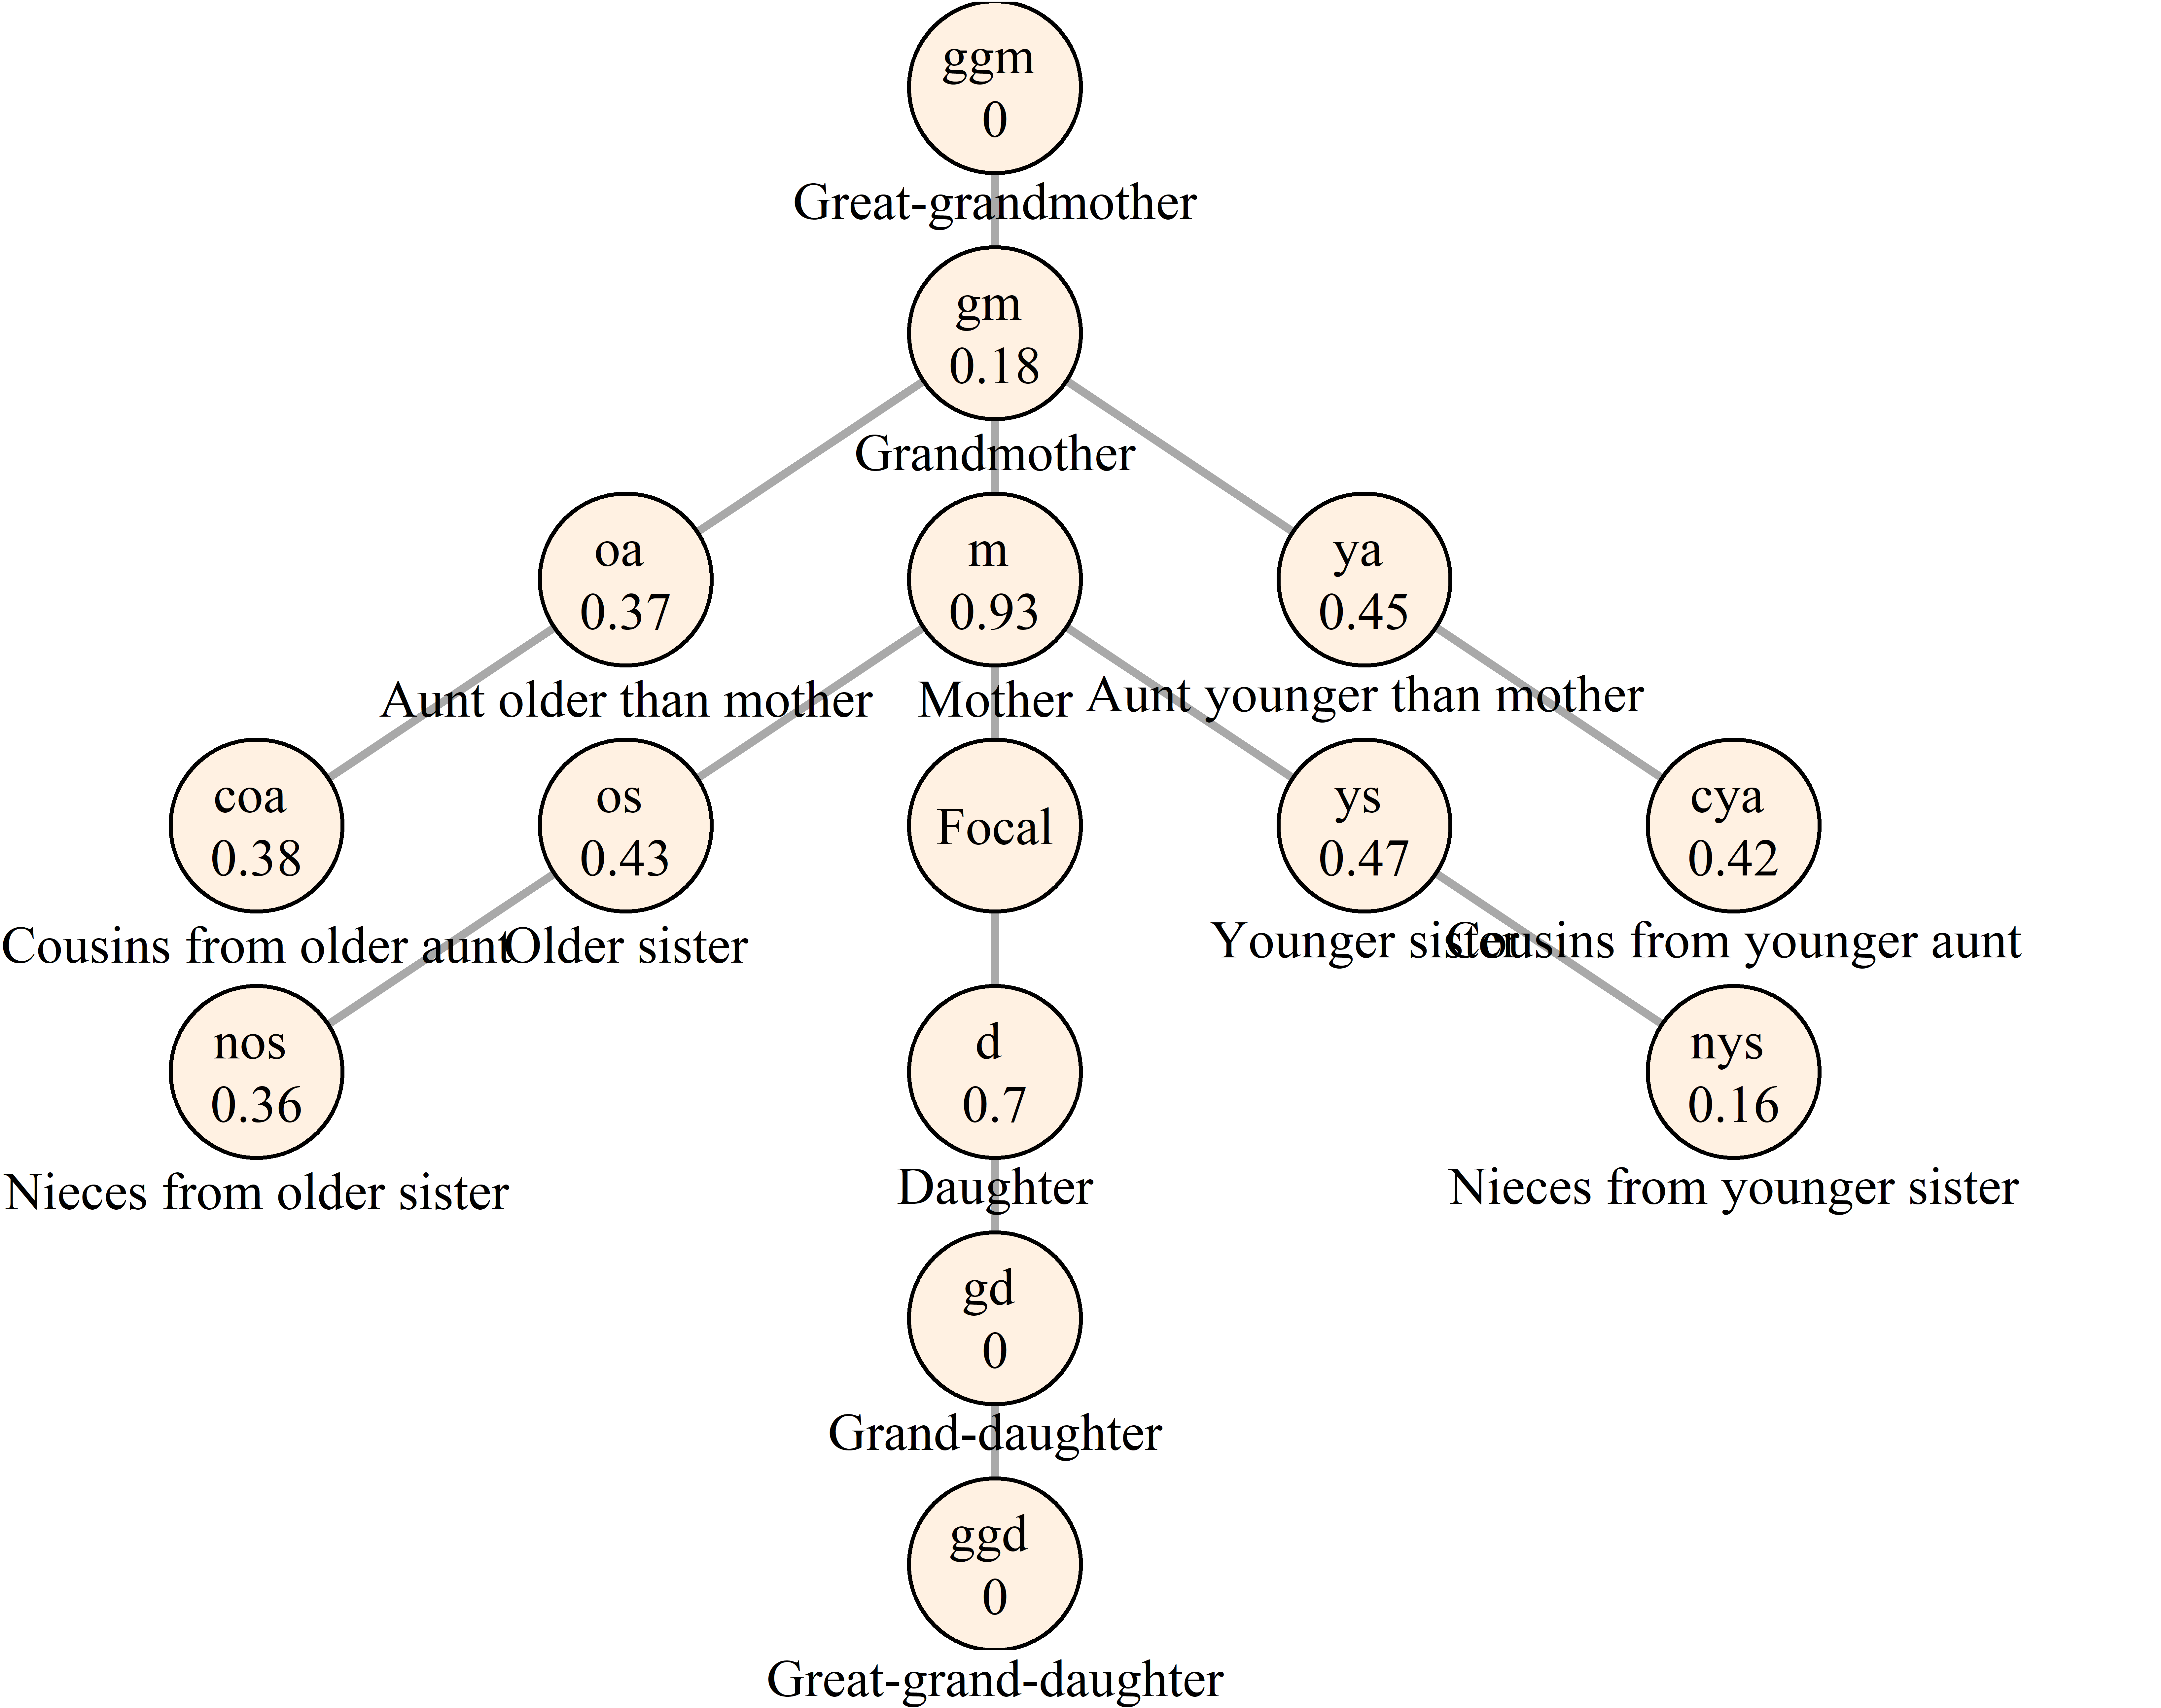
\includegraphics[width =1\textwidth]{figures/tree.png}
     \end{figure}
\end{frame}

\begin{frame}{Demographic subsidy}
    
    \say{New members of the population arise not from reproduction of current members, but from elsewhere}\fcite{caswell_formal_2019}

    \begin{itemize}
        \item Can you think of other instances of `subsidy' in demography?
    \end{itemize}
    
\end{frame}

\begin{frame}{}
    \centering \huge Break
\end{frame}

\section{Matrix kinship models}
\begin{frame}
    \begin{centering}
    \begin{beamercolorbox}[sep=12pt,center]{part title}
    \usebeamerfont{section title}\insertsection\par
    \end{beamercolorbox}
    \end{centering}
\end{frame}

\begin{frame}{From recursive equations to matrix operations}
\begin{minipage}{0.7\textwidth}
\begin{enumerate}
        \item The relatives of Focal constitute a population
        \item They can be modelled using traditional projection methods
        \item Matrix operations provide an efficient implementation
    \end{enumerate}
    \end{minipage} \hfill
    \begin{minipage}{0.25\textwidth}
    \begin{figure}[!h]
       \flushright
       
\includegraphics[width =1\textwidth]{figures/ppl.JPG}
     \end{figure}
    \end{minipage}
\end{frame}

\begin{frame}{The tree of life (2)}
       \begin{figure}[!h]
       \centering
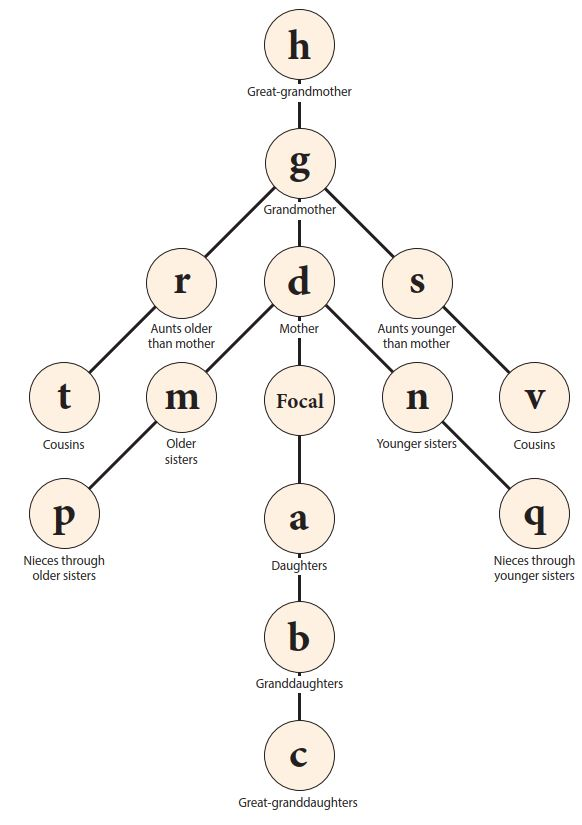
\includegraphics[width =.5\textwidth]{figures/cas_kin.JPG}
     \end{figure}
\end{frame}

\begin{frame}{Implementation: time-invariant, one-sex models\fcite{caswell_formal_2019}}
    The models are of the general form:

\begin{equation*}
    	\underbrace{{\bf k}(x+1)}_{\substack{\text{age structure of kin}\\ \text{at Focal's age $x+1$}}} = 	
    \underbrace{{\bf U \, k}(x)}_{\substack{\text{ageing and survival}\\ \text{of existing kin}}}
    + 	\underbrace{	\left\{ \begin{array}{l}
    \bm 0 \\
    {\bf F \, k}^*(x)
    \end{array}
    \right.}_{\substack{\text{new kin members}\\ \text{added to the population}}}.
\end{equation*}

where:
\vspace{.2cm}
\begin{itemize}
    \item ${\bf U}$ a matrix with survival probabilities in the subdiagonal
    \item ${\bf F}$ a matrix with fertility rates in the first row
\end{itemize}
\end{frame}

\begin{frame}{Age distributions of kin}
    \begin{figure}[!h]
       \centering
        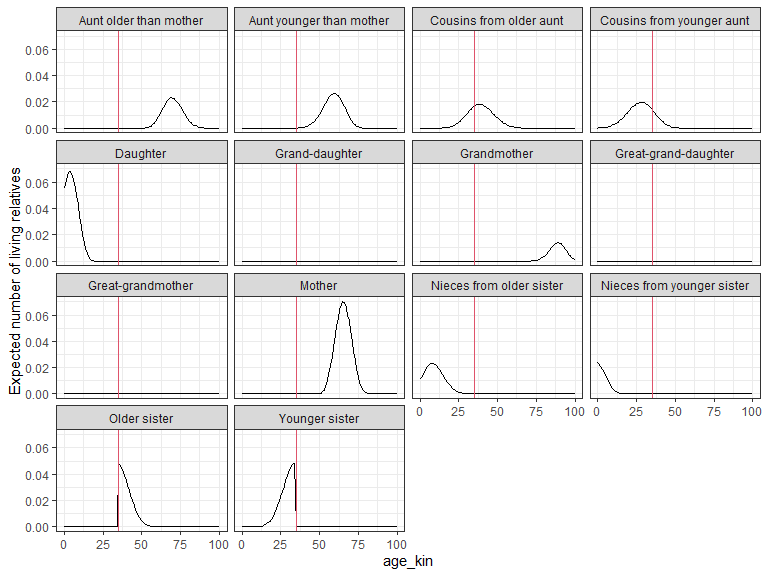
\includegraphics[width =1\textwidth]{figures/kin2.png}
     \end{figure}
\end{frame}

\begin{frame}{Expected number of kin}
    \begin{figure}[!h]
       \centering
        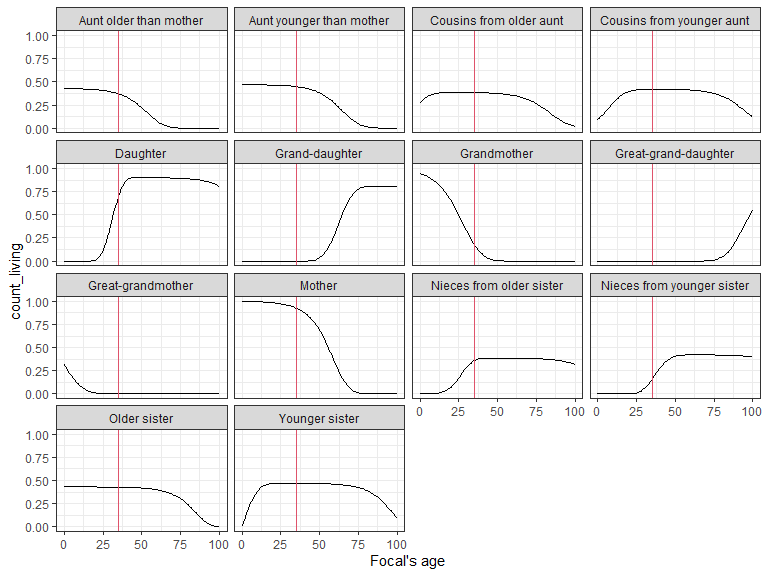
\includegraphics[width =1\textwidth]{figures/kin1.png}
     \end{figure}
\end{frame}

\begin{frame}{Daughters}

Daughters ($\bf a$) are the result of the reproduction of Focal:

    \begin{equation}
    	\underbrace{{\bf a}(x+1)}_{\substack{\text{age structure of daughters}\\ \text{at Focal's age $x+1$}}} = 	
    \underbrace{{\bf U \, a}(x)}_{\substack{\text{ageing and survival}\\ \text{of existing daughters}}}
    + 	\underbrace{	{\bf F \, e}_x.}_{\substack{\text{new daughters}\\ \text{(subsidy)}}}
\end{equation}

\begin{equation*}
    a(0) = {\bf 0}.
\end{equation*}

where:
\begin{itemize}
    \item ${\bf U}$ is a matrix with survival probabilities in the subdiagonal
    \item ${\bf F}$ is a matrix with fertility rates in the first row
    \item ${\bf F \, e}_x$ is the subsidy vector
    \item $e_x$ is the unit vector for age $x$
    \item $a(0)$ is the distribution of daughters at Focal's birth
\end{itemize}

\end{frame}

\begin{frame}{Mothers}

 The population of mothers ($\bf d$) of Focal consists of at most a single
individual:

    \begin{equation}
    	\underbrace{{\bf d}(x+1)}_{\substack{\text{age structure of mothers}\\ \text{at Focal's age $x+1$}}} = 	
    \underbrace{{\bf U \, d}(x)}_{\substack{\text{ageing and survival}\\ \text{of existing mothers}}}
    + 	\underbrace{	{\bf 0}.}_{\substack{\text{new mothers}\\ \text{(subsidy)}}}
\end{equation}

\begin{equation*}
    d(0) = {\bf \pi}.
\end{equation*}

where:
\begin{itemize}
    \item $b(0)$ is the distribution of mothers at Focal's birth
    \item ${\bf \pi}$ is the distribution of ages of mothers in the population
\end{itemize}

\end{frame}

\begin{frame}{All models\fcite{caswell_formal_2019}}
       \begin{figure}[!h]
       \centering
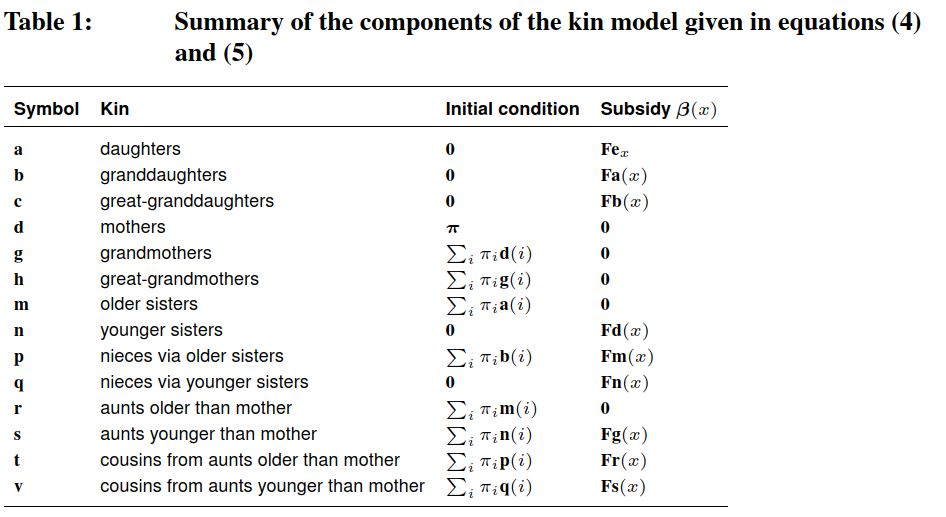
\includegraphics[width =1\textwidth]{figures/kin-sum.JPG}
     \end{figure}
\end{frame}


 \begin{frame}{Consider a  baby born in Spain in 1950...}
     \begin{enumerate}
         \item How old were her grandparents when she was born, on average?
         \item How many living children did she have on her 70th birthday?
         \item How many grandchildren?
     \end{enumerate}
 \end{frame}

\begin{frame}{}
    \centering \huge Break
\end{frame}


\section{Implementations}
\begin{frame}
    \begin{centering}
    \begin{beamercolorbox}[sep=12pt,center]{part title}
    \usebeamerfont{section title}\insertsection\par
    \end{beamercolorbox}
    \end{centering}
\end{frame}

\begin{frame}{Total number of kin (all kin combined) for a 5yo woman\fcite{alburez-gutierrez_projections_2023}}
       \begin{figure}[!h]
       \centering
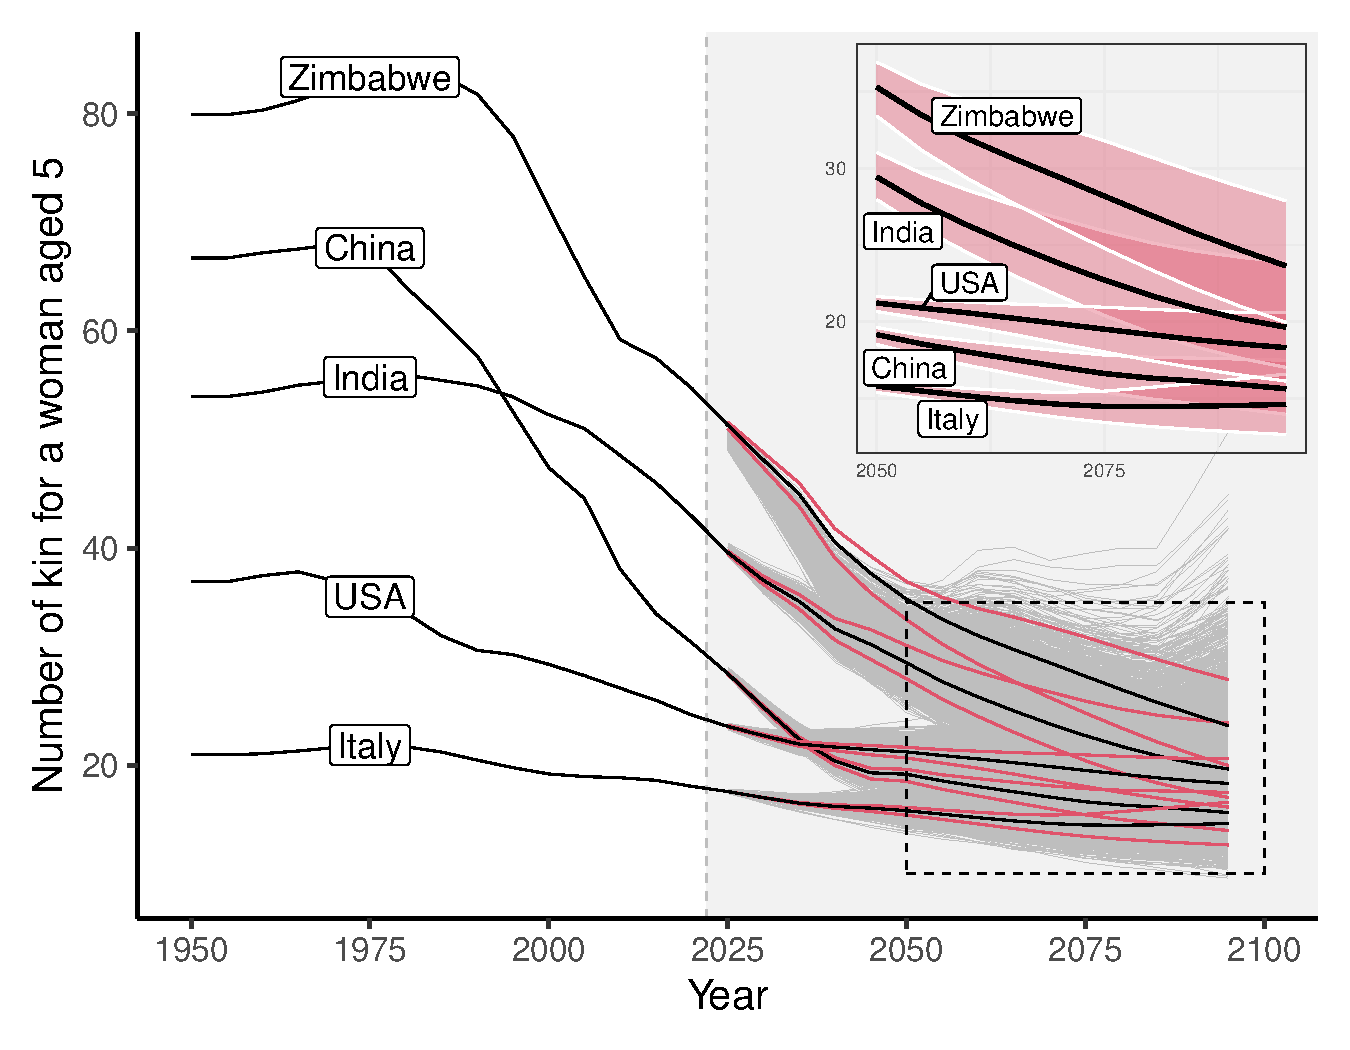
\includegraphics[width =.9\textwidth]{figures/kin_forecast_trajectories2.pdf}
     \end{figure}
\end{frame}

\begin{frame}{Number of living kin for a 65yo in China}
       \begin{figure}[!h]
       \centering
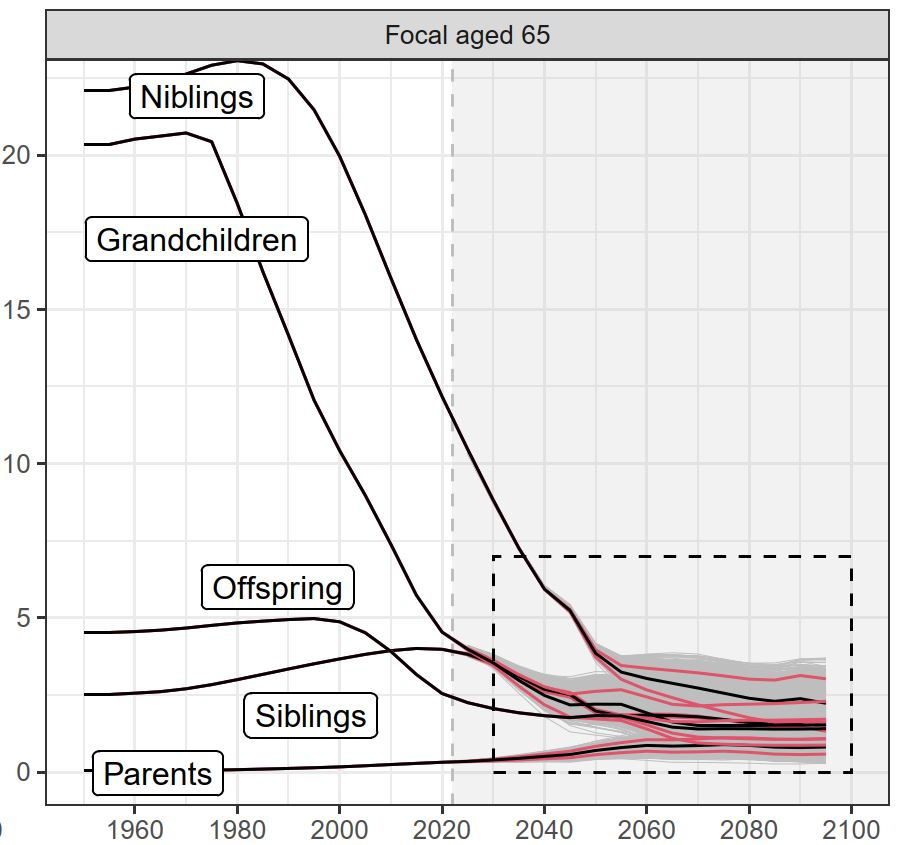
\includegraphics[width =.75\textwidth]{figures/wpp_kin_traj4.2.JPG}
     \end{figure}
\end{frame}


\begin{frame}{Models vs reality}
    Discuss:
    \begin{enumerate}
        \item What is the relationship between demographic models and reality?
        \item Would we expect kinship models to agree with `empirical' observations of kinship?
        \item Where can we find empirical data on kinship availability?
    \end{enumerate}
\end{frame}

\end{document}



